\documentclass[handout]{beamer}
\usetheme{cambridge}

\usepackage[english]{babel}
\usepackage[latin1]{inputenc}

\usepackage{graphicx}
%\usepackage{enumitem}

% Author, Title, etc.
\title{Bayesian optimisation of approximateness in the trade-off between statistical and computational efficiency}
\author{Jan S\"ondermann}
\institute{University of Cambridge}


\begin{document}

\begin{frame}
  \titlepage
\end{frame}


\begin{frame}{Introduction}
\begin{itemize}
\item<1-> Since advent of computers, complex new statistical methods have been developed
\item<2-> Many of these methods are slow or even intractable on current computers
\item<3-> ``Big data" is a trend that exacerbates this problem
%\item<4-> Illustrated by different perspectives on data in statistics/computer science
\item<4-> Experts make decisions about when to use approximations
\item<5-> This should be automated
\end{itemize}
\end{frame}

\begin{frame}{Introduction}
\begin{itemize}
\item<1-> Runtime considerations not traditionally in the focus of statistical research

\item<2-> Different perspectives on data:
\begin{itemize}
\item<3-> \textbf{Statistics}: more data is better, allows higher confidence in results
\item<4-> \textbf{Computer science}: data is a workload to be completed
\end{itemize}
%\item<5-> The computer science perspective is still lacking in machine learning %TODO
\end{itemize}
\end{frame}

\begin{frame}{Introduction}
\begin{itemize}
\item<1-> Many different possible goals when adding runtime considerations
%\begin{itemize}
\item<2-> Anytime algorithm
\item<3-> Contract algorithm
\item<4-> Accuracy fixed
%\end{itemize}
\item<5-> $\cdots$
\end{itemize}
\end{frame}

\begin{frame}{Approximation parameters}
\begin{itemize}
\item<1-> Approximation parameters to learning algorithm control degree of approximateness
\item<2-> Functions from approximation parameters to runtime and predictive accuracy
\item<3-> Model of these functions
\end{itemize}
\end{frame}

\begin{frame}{Logistic regression/MNIST}
\begin{figure}
  \centering
  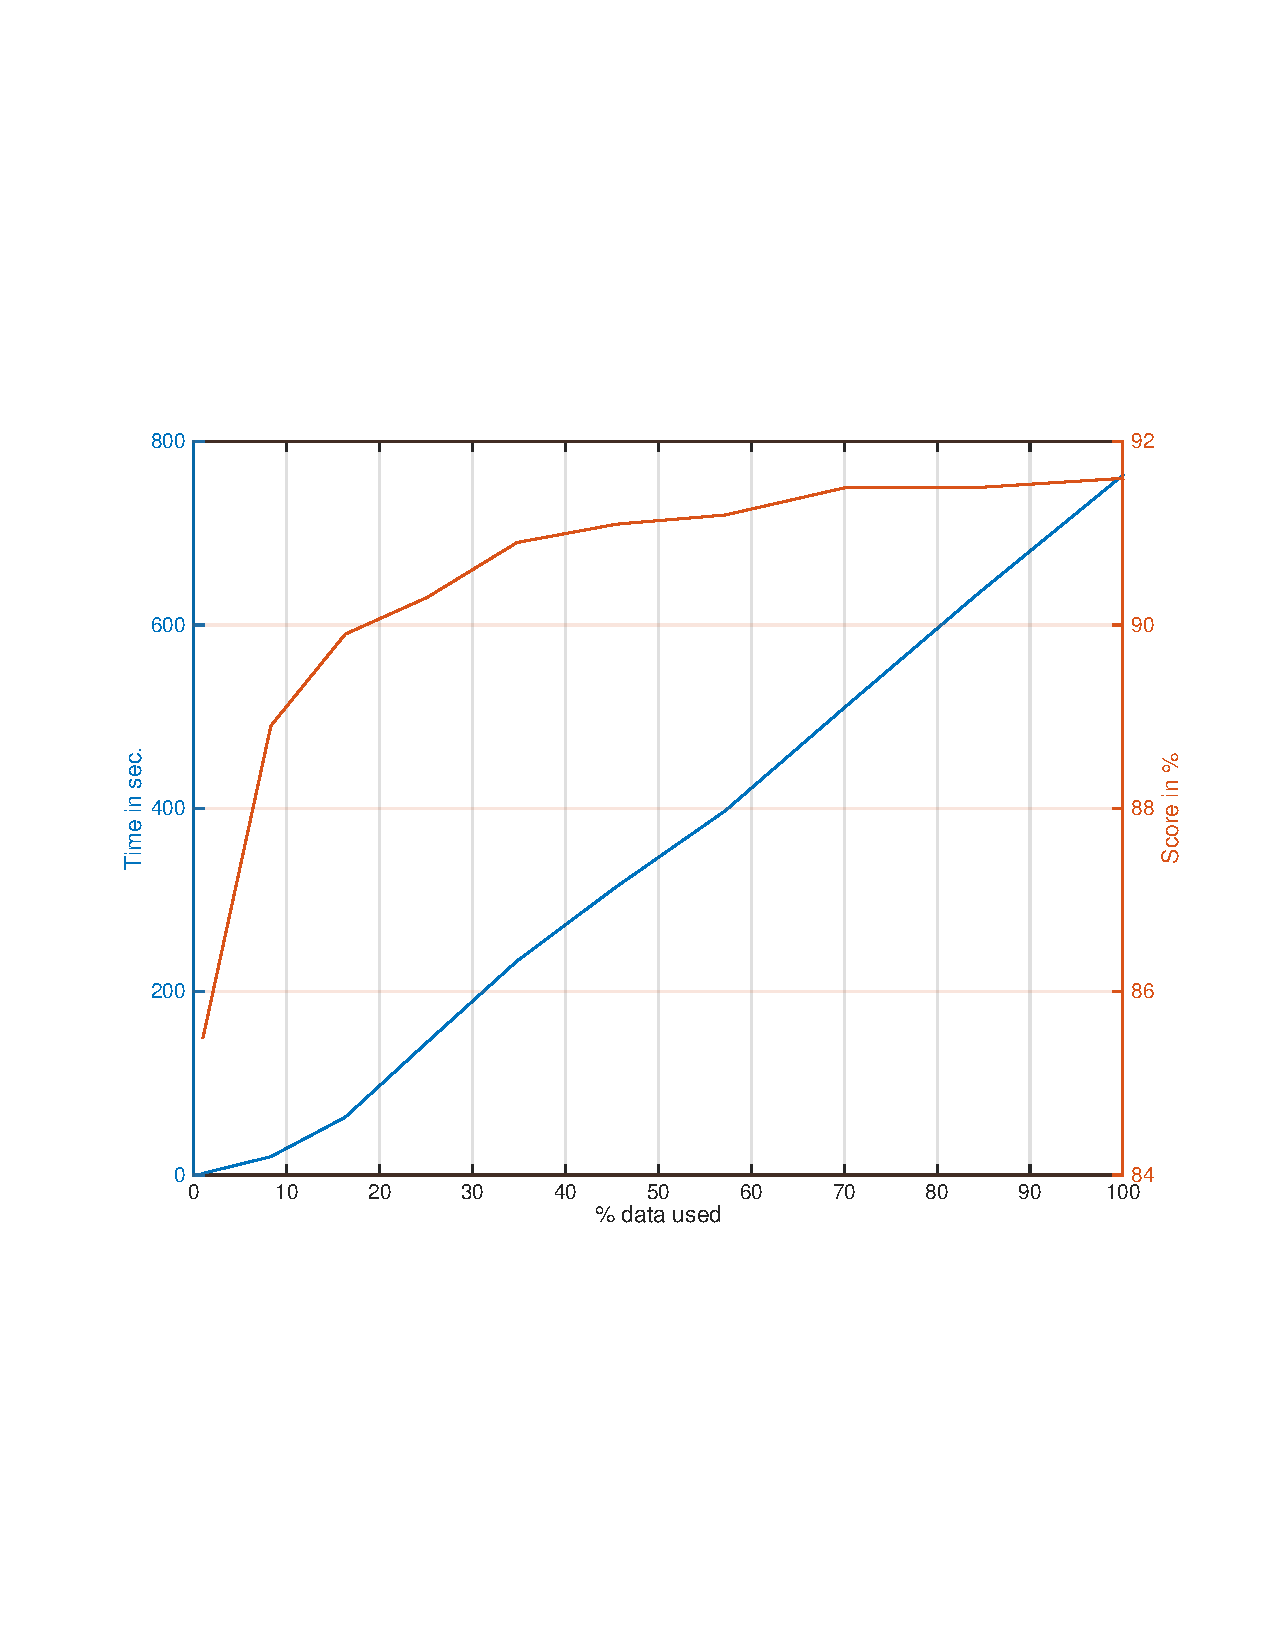
\includegraphics[trim=50 200 35 205,clip,width=.75\linewidth]{lr_mnist.pdf}
  \caption{}
  \label{sampledata1}	
\end{figure}
\end{frame}


\begin{frame}{Random forest/Synthetic data}
\begin{figure}
  \centering
  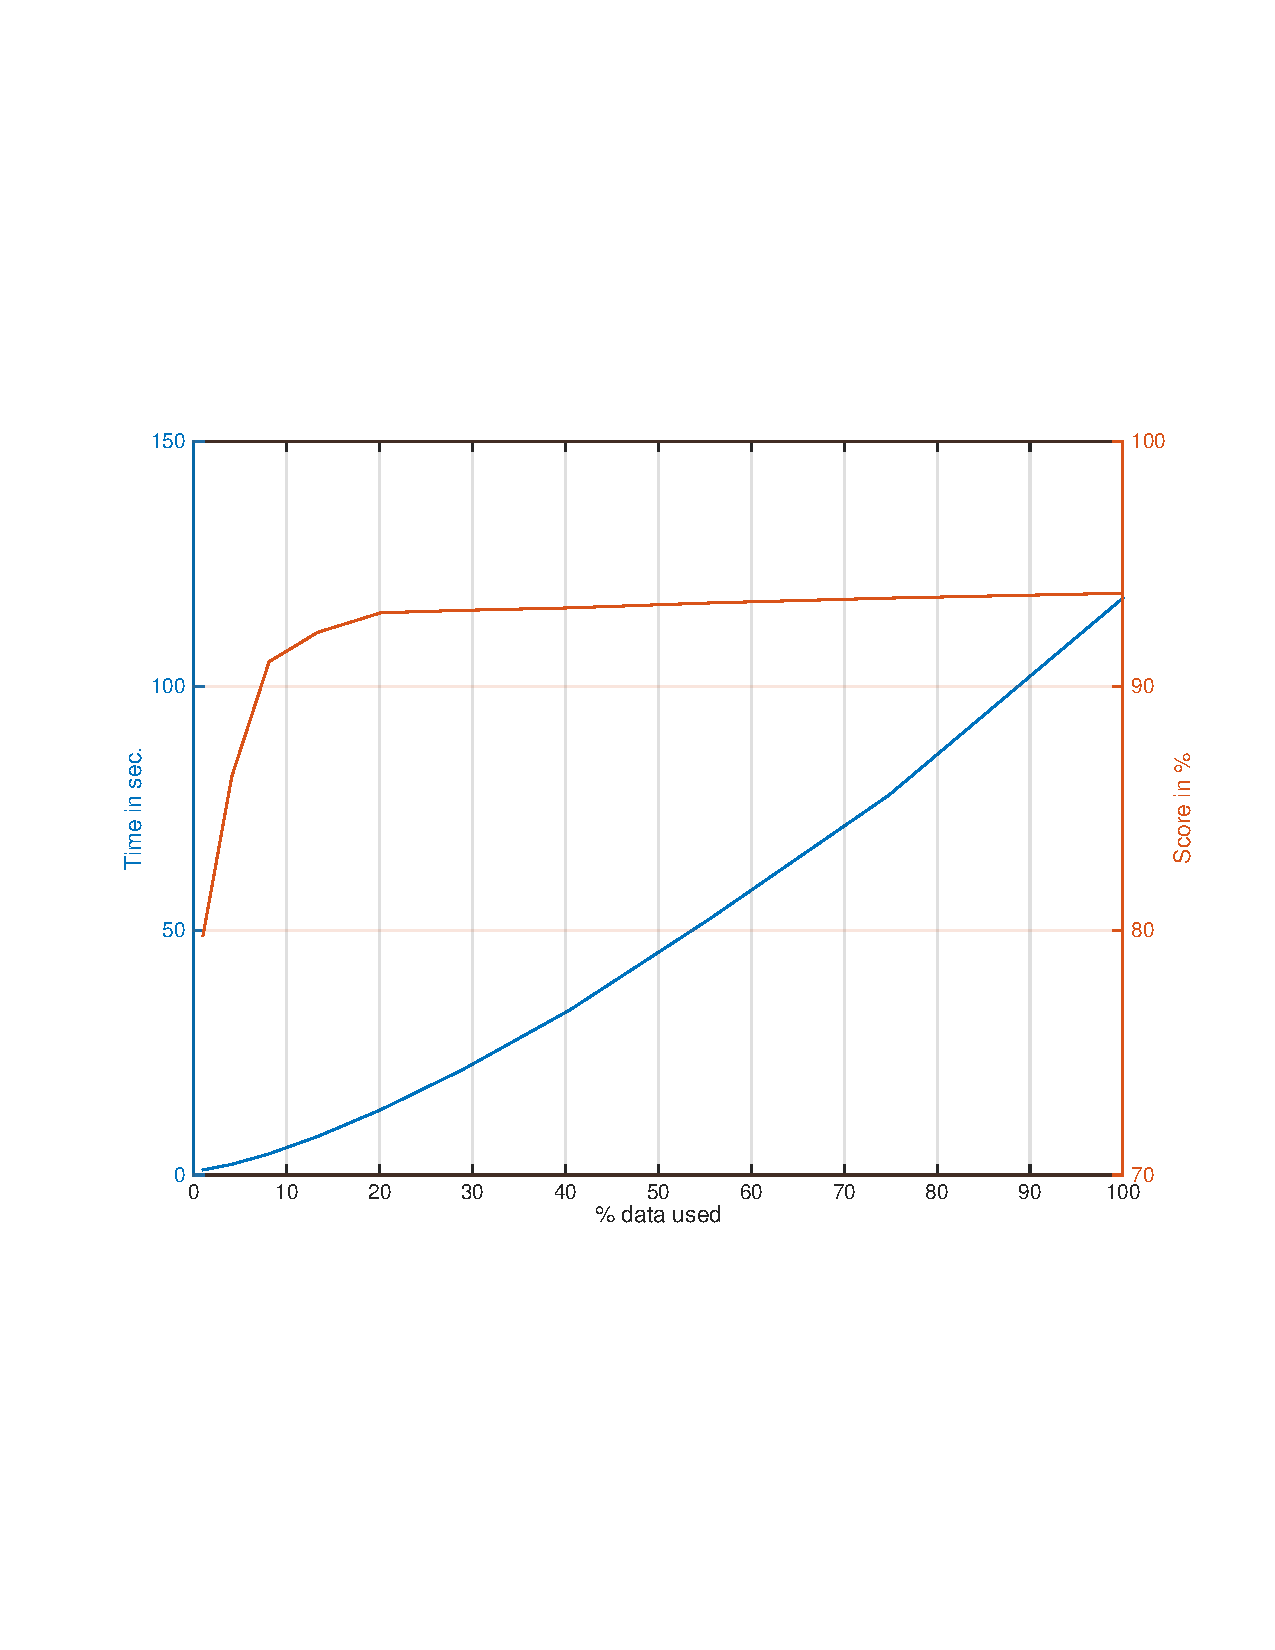
\includegraphics[trim=50 200 35 205,clip,width=.75\linewidth]{rf_synth.pdf}
  \label{sampledata1}	
\end{figure}
\end{frame}

\begin{frame}{Modelling performance}
\begin{figure}
  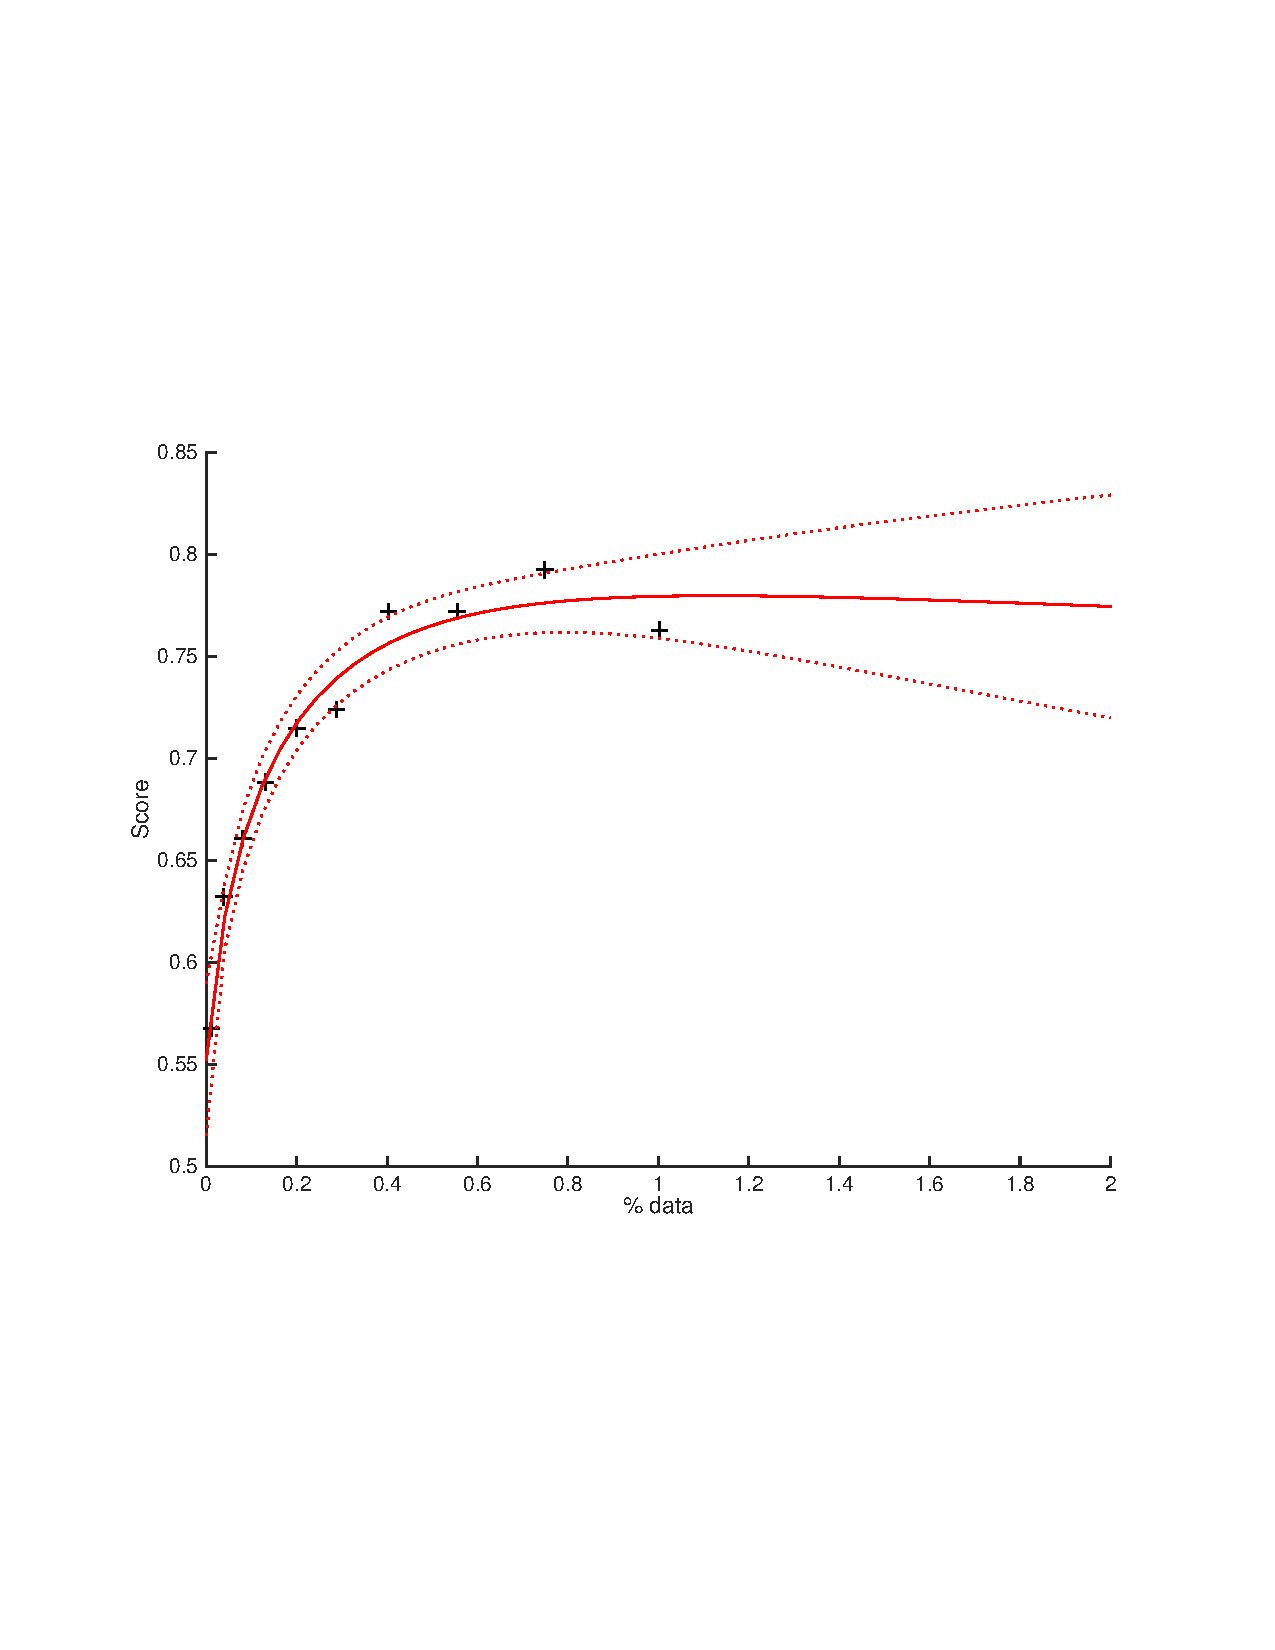
\includegraphics[trim=50 190 50 200,clip,width=.7\textwidth]{synth3_rndforest_fit.pdf}
  \caption{Fits for the Synthetic3 logistic regression score data with the squared exponential fit in blue and the exponential mixture fit in red.}
  \label{synth3_rndforest_fit}
\end{figure}
\end{frame}

\begin{frame}{Optimisation}
	\begin{itemize}
		\item<1-> Finding approximateness trade-off is an optimisation problem
		\item<2-> Function potentially very costly to evaluate
		\item<3-> Natural candidate: Bayesian optimisation
		\begin{itemize}
			\item<4-> Efficient in number of evaluations
			\item<5-> Making decisions comparatively costly
		\end{itemize}
		\item<6-> Expected improvement: balancing exploration \& exploitation
		\item<7-> Modified to take runtime into account leading to a set of heuristics
	\end{itemize}
\end{frame}


\begin{frame}{Anytime heuristic}
\begin{itemize}
\item Expected improvement $\cdot$ probability of finishing in time	
\end{itemize}

\begin{figure}
\centering
  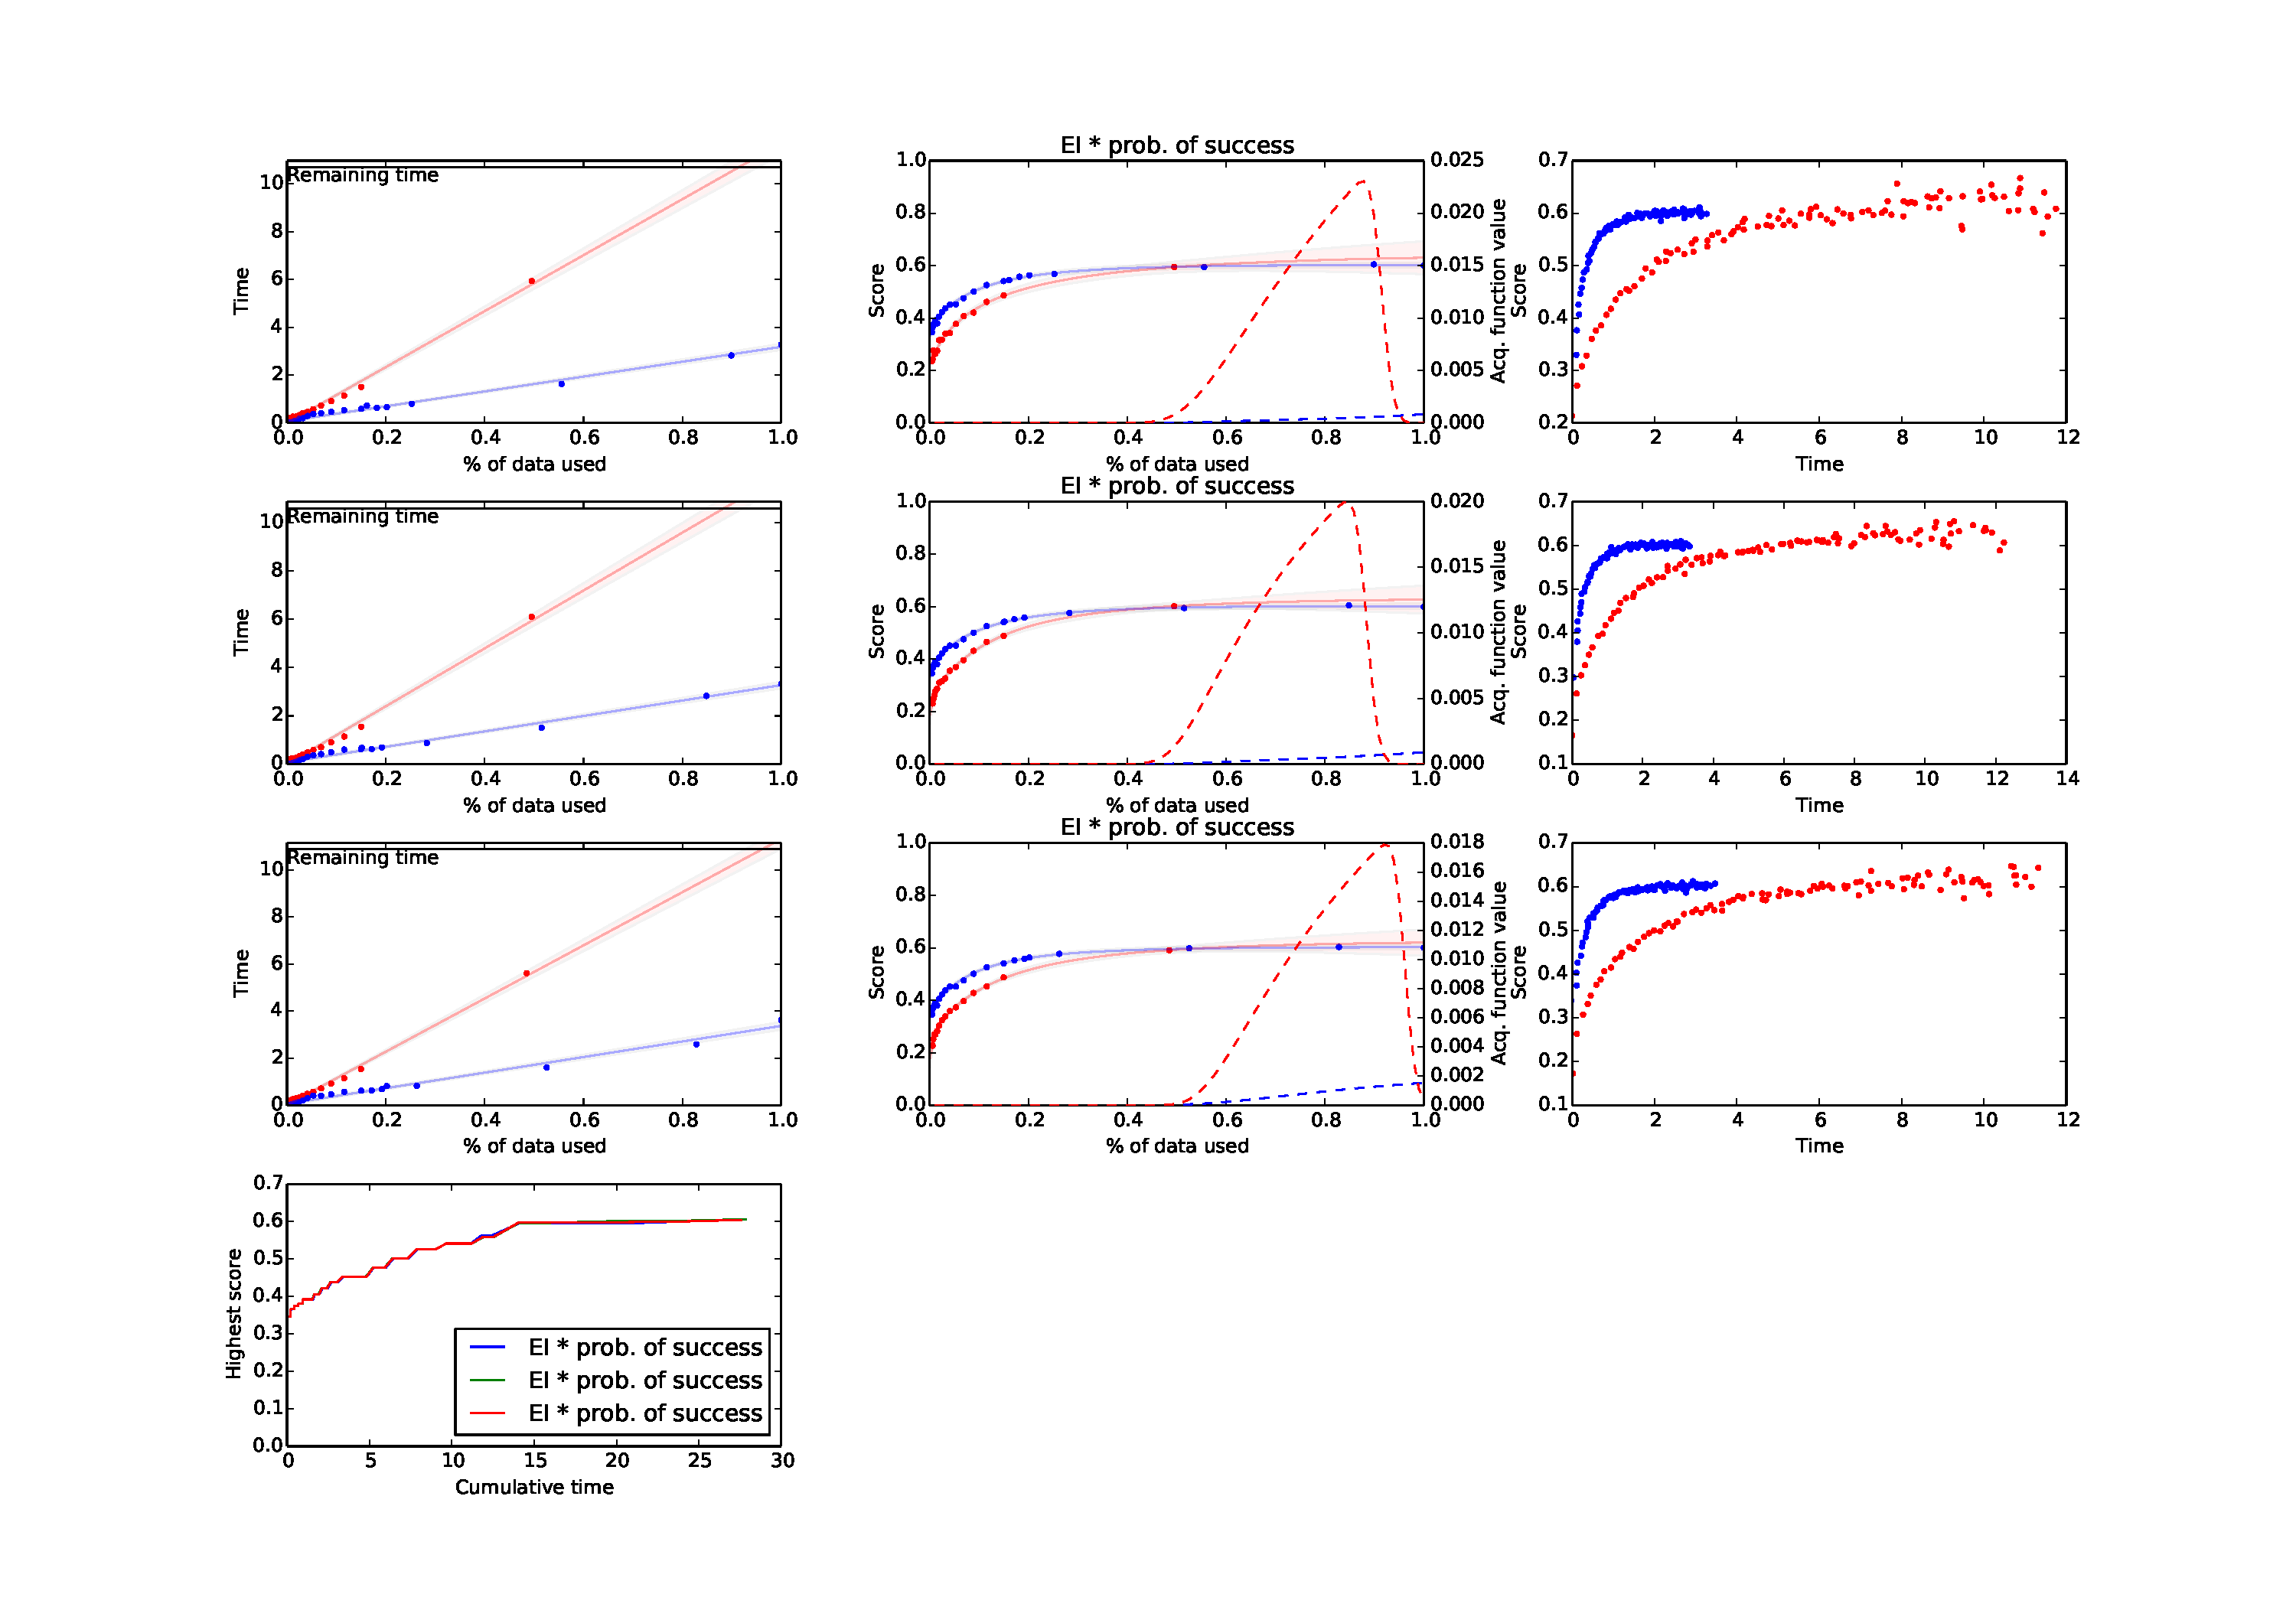
\includegraphics[trim=140 710 493 55,clip,width=\textwidth]{ei_probofsuccess2.pdf}
  \label{sched:expimprpertime02}
\end{figure}
\end{frame}

\begin{frame}{Anytime heuristic}
\begin{figure}
\centering
  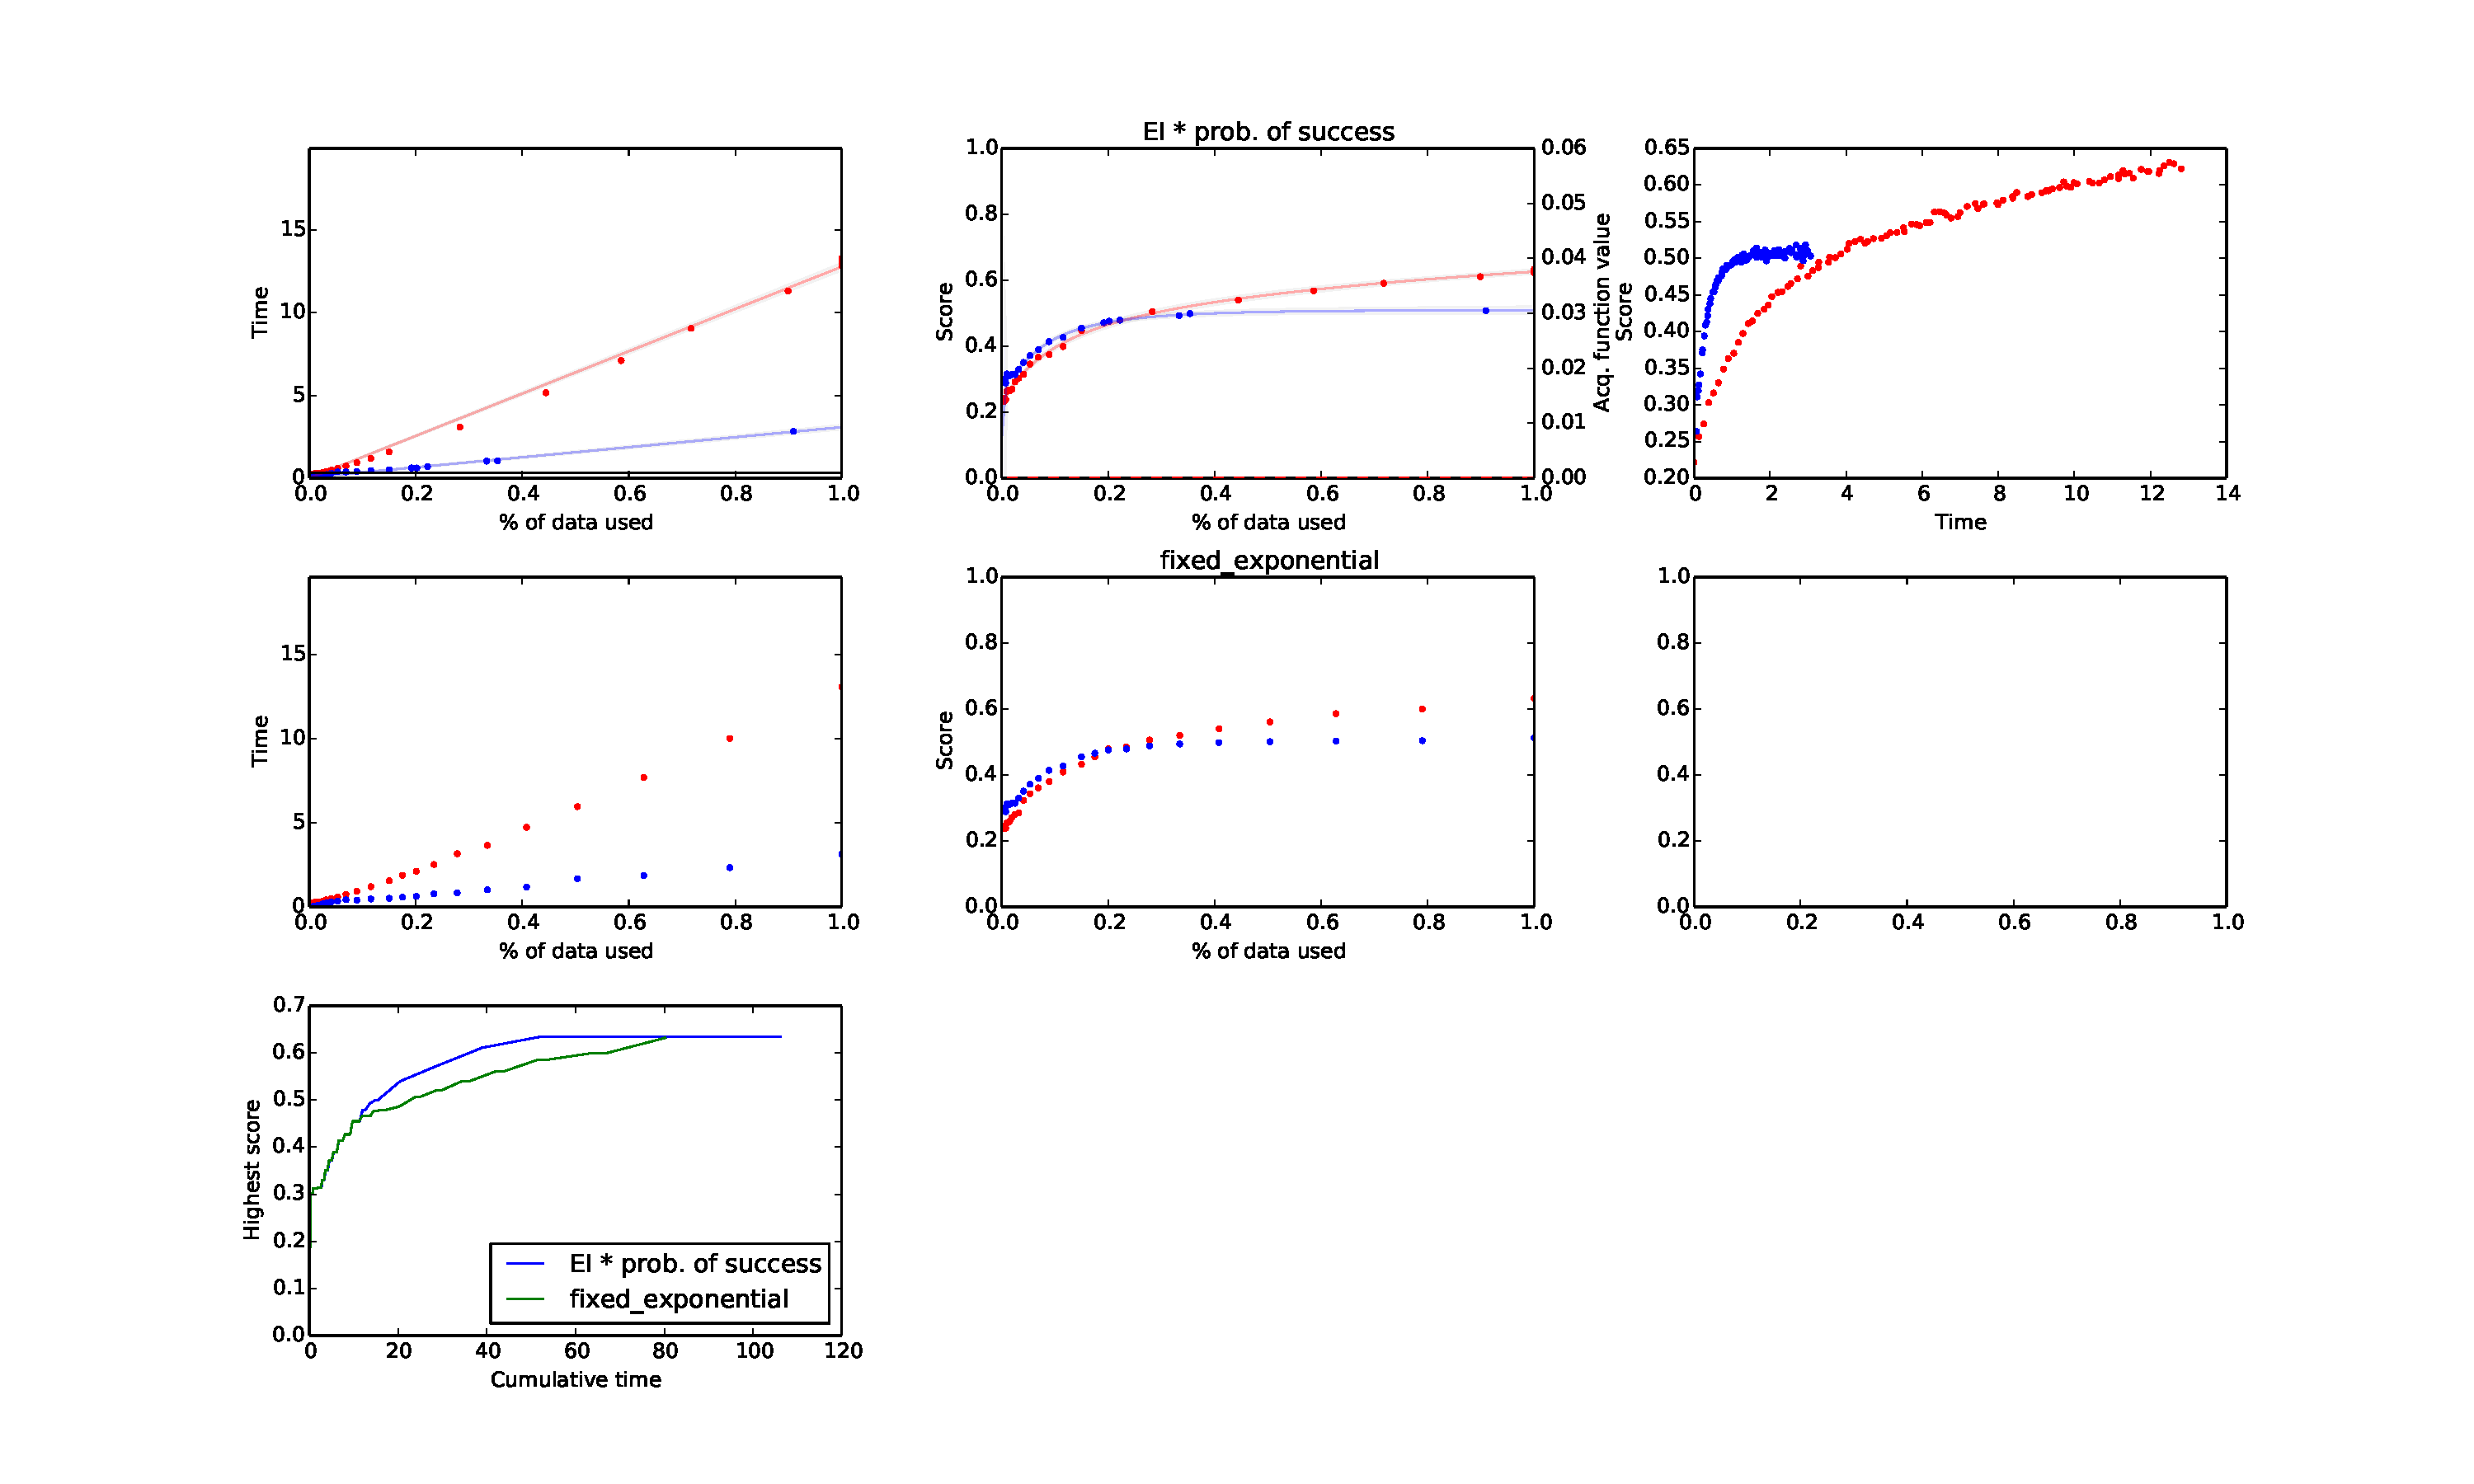
\includegraphics[trim=130 40 930 570,clip,width=.8\textwidth]{anytime1.pdf}
  \label{anytime1}
\end{figure}
\end{frame}

\begin{frame}{Contract heuristic}
\begin{itemize}
\item One time budget to explore, one to exploit	
\end{itemize}

\begin{figure}
\centering
  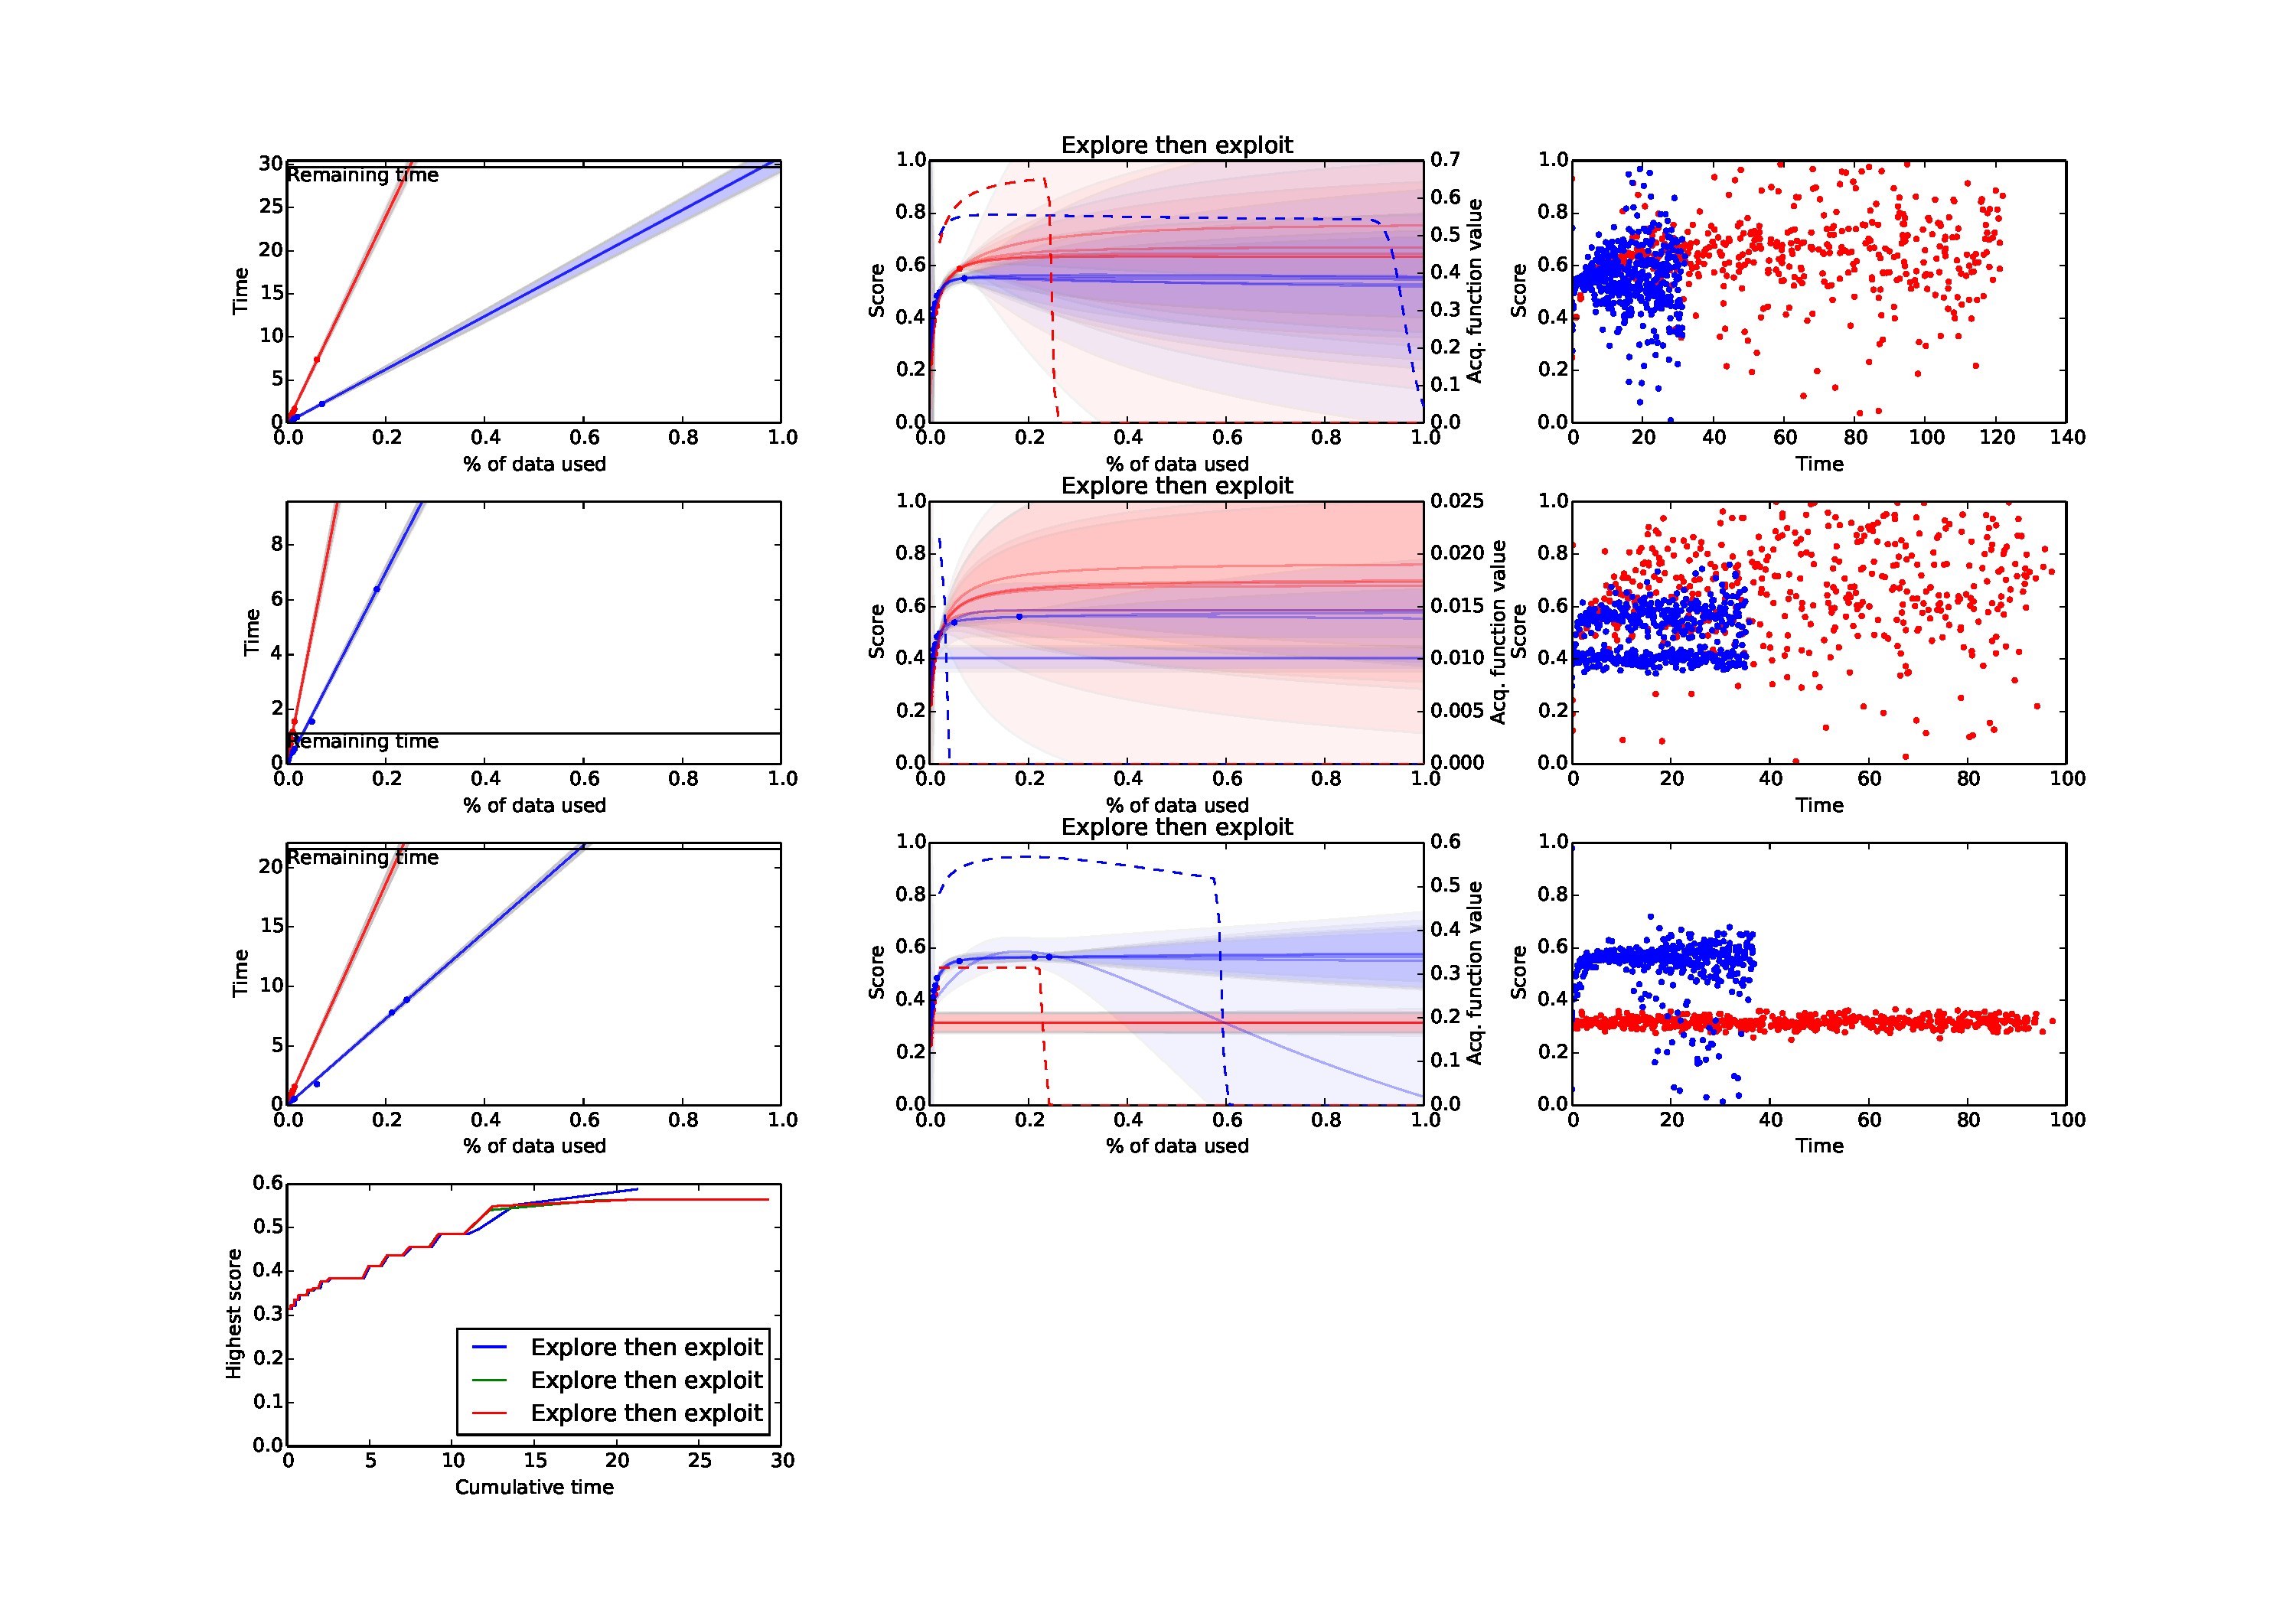
\includegraphics[trim=140 710 493 55,clip,width=\textwidth]{exp_then_exp3.pdf}

  \label{sched:exp_then_exp3}
\end{figure}
\end{frame}

\begin{frame}{Conclusion}
\begin{itemize}
\item<1-> Approximation parameters to learning algorithms
\item<2-> Modelling algorithm performance with Gaussian processes
\item<3-> Bayesian optimisation of approximation function
\item<4-> Heuristics for anytime/contract style algorithms
\end{itemize}
\end{frame}


\begin{frame}{Questions}

\begin{center}
\Huge Questions?
\end{center}

\end{frame}




\end{document}


